\documentclass[oneside,final]{hcmut-report}
\usepackage{codespace}
\usepackage{gensymb,textcomp}
\usepackage{array,longtable,multicol,multirow,siunitx,tabularx}
\usepackage{enumitem}
\usepackage{caption,float}
\usepackage[export]{adjustbox}
\usepackage[nameinlink]{cleveref}
\usepackage{fancyhdr}
\usepackage{lastpage}
\usepackage{xcolor}

\pagestyle{fancy}
\fancyhf{}
\fancyhead[L]{%
    \begin{tabular}[b]{@{}l@{}}
        Ho Chi Minh City University of Technology \\
        Faculty of Computer Science and Engineering
    \end{tabular}%
}
\fancyhead[R]{%
    \raisebox{-0.15\height}{
\includegraphics[height=1.0cm]{graphics/hcmut.png}}%
}
\fancyfoot[C]{\thepage}
\renewcommand{\headrulewidth}{0.4pt}
\renewcommand{\footrulewidth}{0pt}

% ==================== THÔNG TIN BÁO CÁO ====================
\coursename{COMPUTER NETWORK REPORT}
\reporttype{}
\title{Homework 4c}
\advisor{ &}
\stuname{ &}
\reportplace{HO CHI MINH CITY}
\reporttime{NOVEMBER 2026}

\begin{document}

% Trang bìa theo mẫu hcmut-report
\coverpage

% ==================== PAGE 2: QUESTION 1 ====================
\section{Question 1:}
\textbf{Question:} What is the IP address of the client that sends the HTTP GET request in the \textit{nat-inside-wireshark-trace1-1.pcapng} trace? What is the source port number of the TCP segment in this datagram containing the HTTP GET request? What is the destination IP address of this HTTP GET request? What is the destination port number of the TCP segment in this datagram containing the HTTP GET request?

\textbf{Answer:} Looking at packet number 4:
\begin{itemize}[noitemsep]
    \item \textbf{Client IP address (Source IP):} \texttt{192.168.10.11}
    \item \textbf{TCP Source Port:} \texttt{53924}
    \item \textbf{Destination IP address:} \texttt{138.76.29.8}
    \item \textbf{TCP Destination Port:} \texttt{80}
\end{itemize}

\begin{figure}[H]
    \centering
    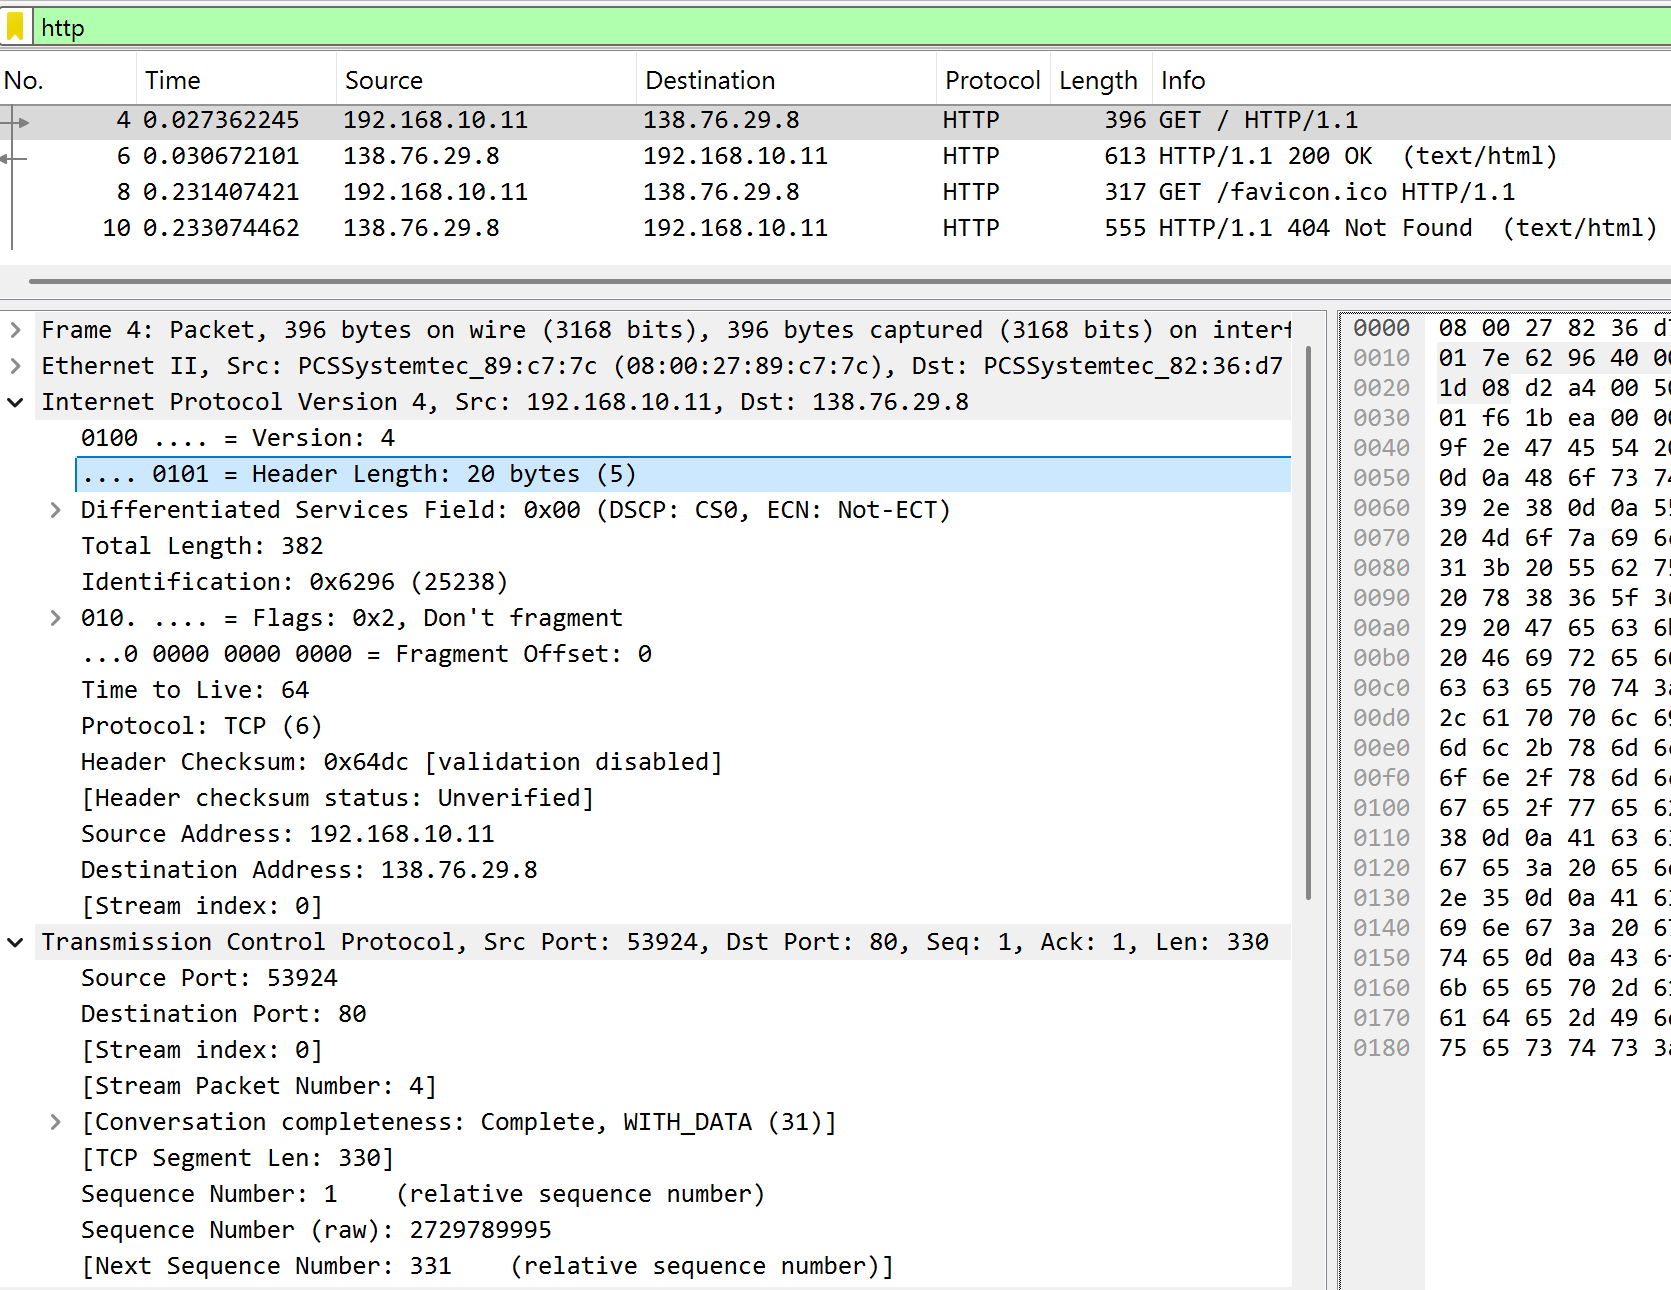
\includegraphics[width=0.58\linewidth]{graphics/fig1_1(2).png}
    \caption{}
\end{figure}


% ==================== PAGE 3: QUESTION 2 & 3 ====================
\section{Question 2:}
\textbf{Question:} At what time is the corresponding HTTP 200 OK message from the webserver forwarded by the NAT router to the client on the router's LAN side?

\textbf{Answer:} The corresponding HTTP 200 OK reply from the web server is packet 6.
The time at which this packet is \textbf{0.030672 seconds}.

\begin{figure}[H]
    \centering
    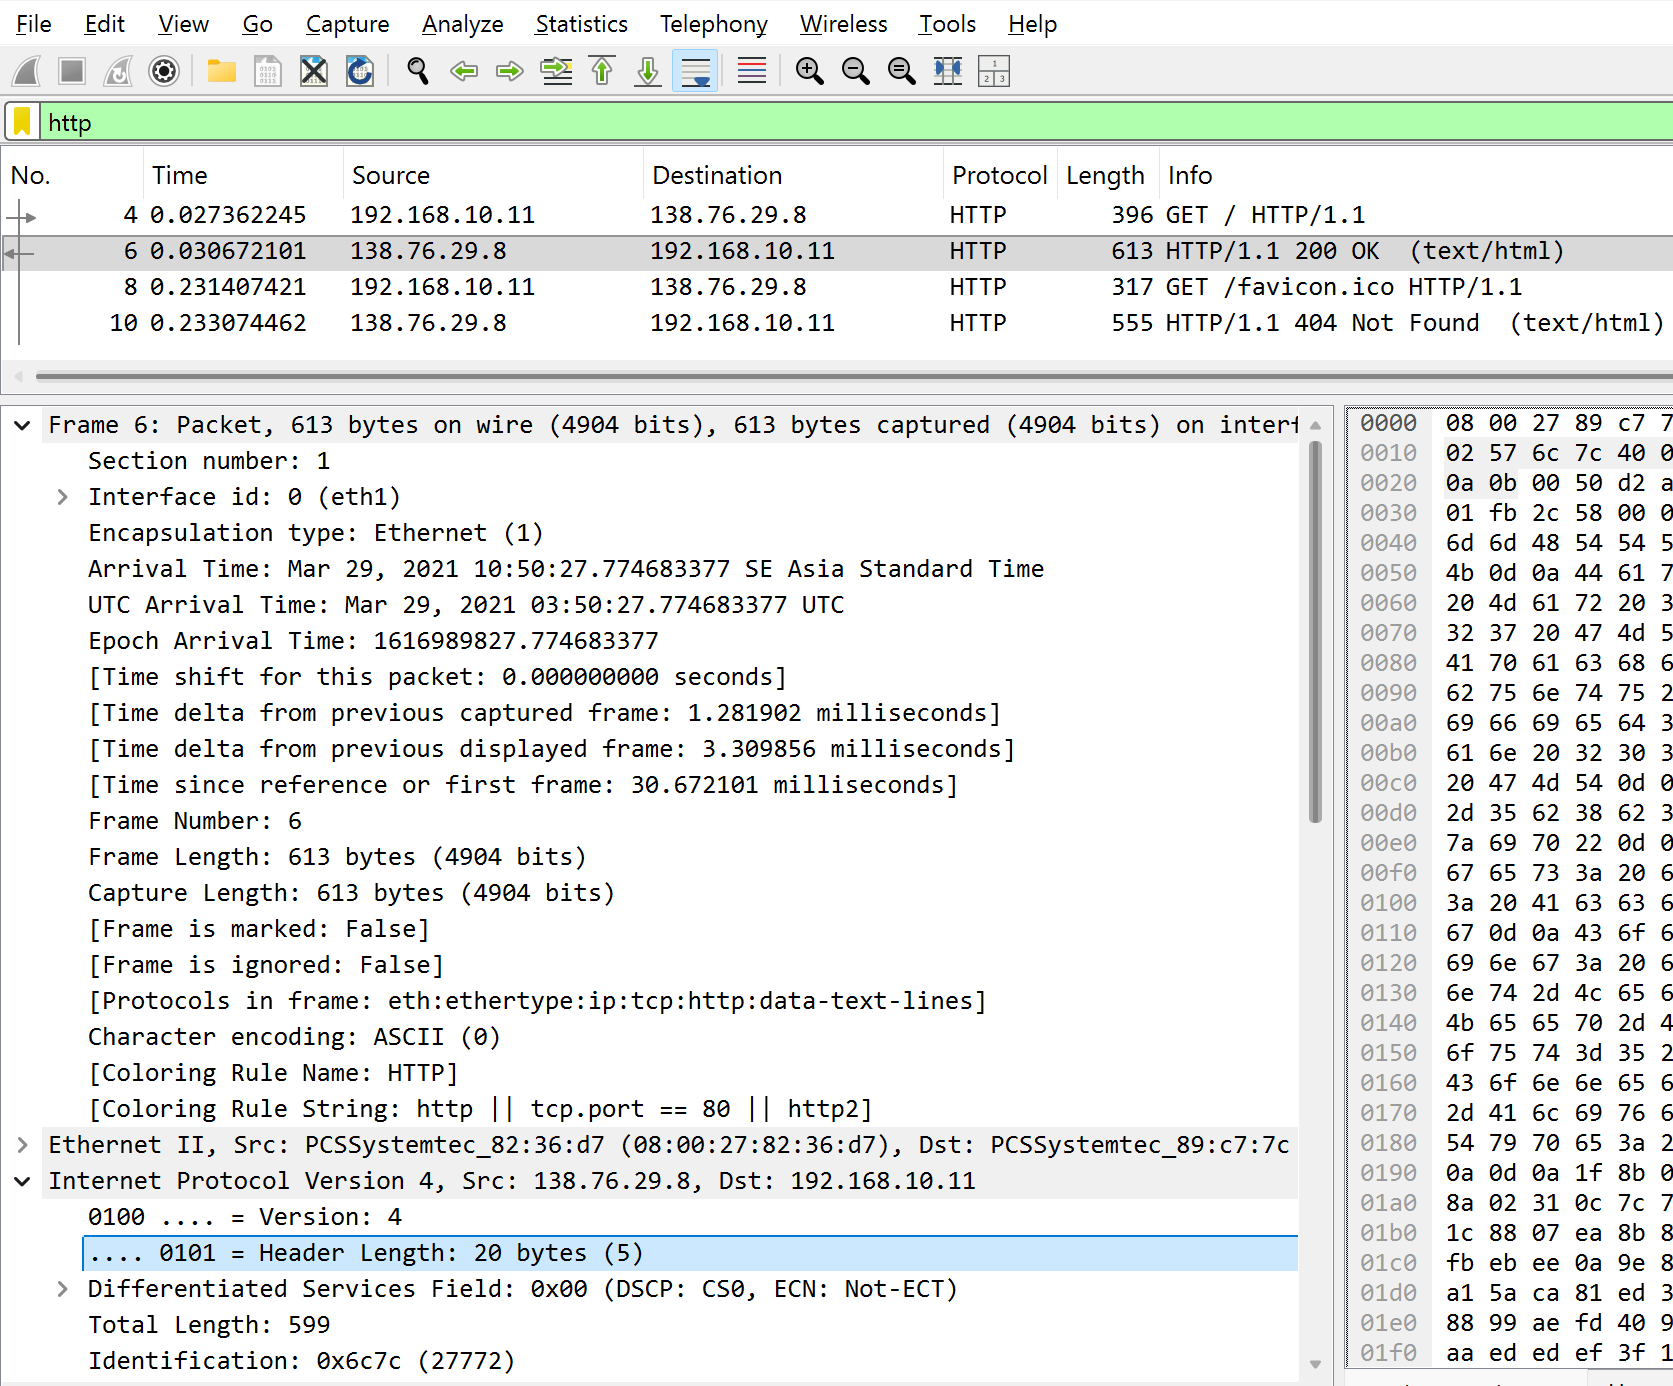
\includegraphics[width=0.58\linewidth]{graphics/fig2_1(2).png}
    \caption{}
\end{figure}

\section{Question 3:}
\textbf{Question:} What are the source and destination IP addresses and TCP source and destination ports on the IP datagram carrying this HTTP 200 OK message?

\textbf{Answer:} At packet number 6:
\begin{itemize}[noitemsep]
    \item \textbf{Source IP address:} \texttt{138.76.29.8}
    \item \textbf{Destination IP address:} \texttt{192.168.10.11}
    \item \textbf{TCP Source port:} \texttt{80}
    \item \textbf{TCP Destination port:} \texttt{53924}
\end{itemize}
\textbf{Relationship between port numbers and IP addresses:} The IP addresses and TCP port numbers are swapped compared to the HTTP GET request in Question 1, as this packet travels in the reverse direction (from the external web server back to the internal LAN client).

\begin{figure}[H]
    \centering
    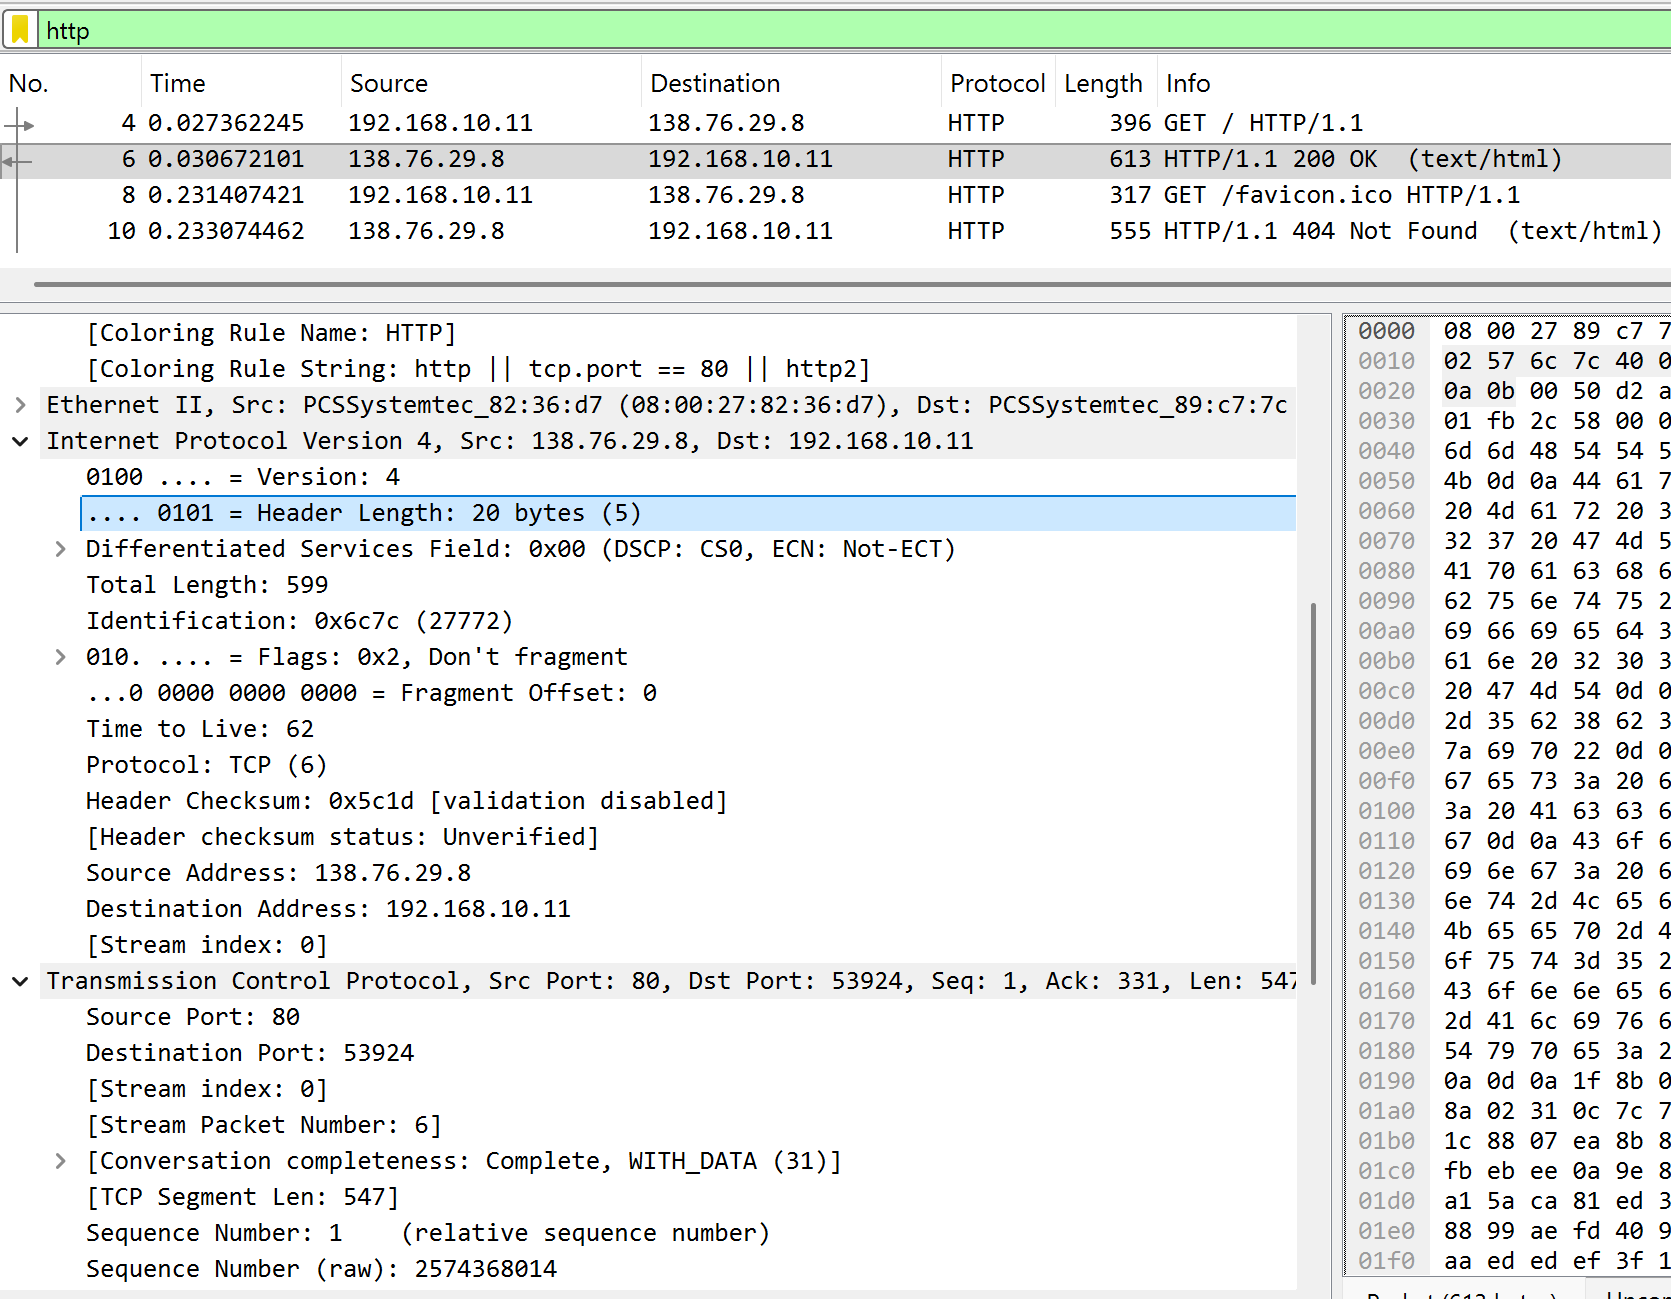
\includegraphics[width=0.58\linewidth]{graphics/fig2_2.png}
    \caption{}
\end{figure}


% ==================== PAGE 4: QUESTION 4, 5, 6 ====================
\section{Question 4:}
\textbf{Question:} At what time does this HTTP GET message appear in the \textit{nat-outside-wireshark-trace1-1.pcapng} trace file?

\textbf{Answer:} The HTTP GET message corresponding to the request sent by the client appears as packet number 4.
The time at which this message appears in the outside trace is \textbf{0.027356 seconds}.

\begin{figure}[H]
    \centering
    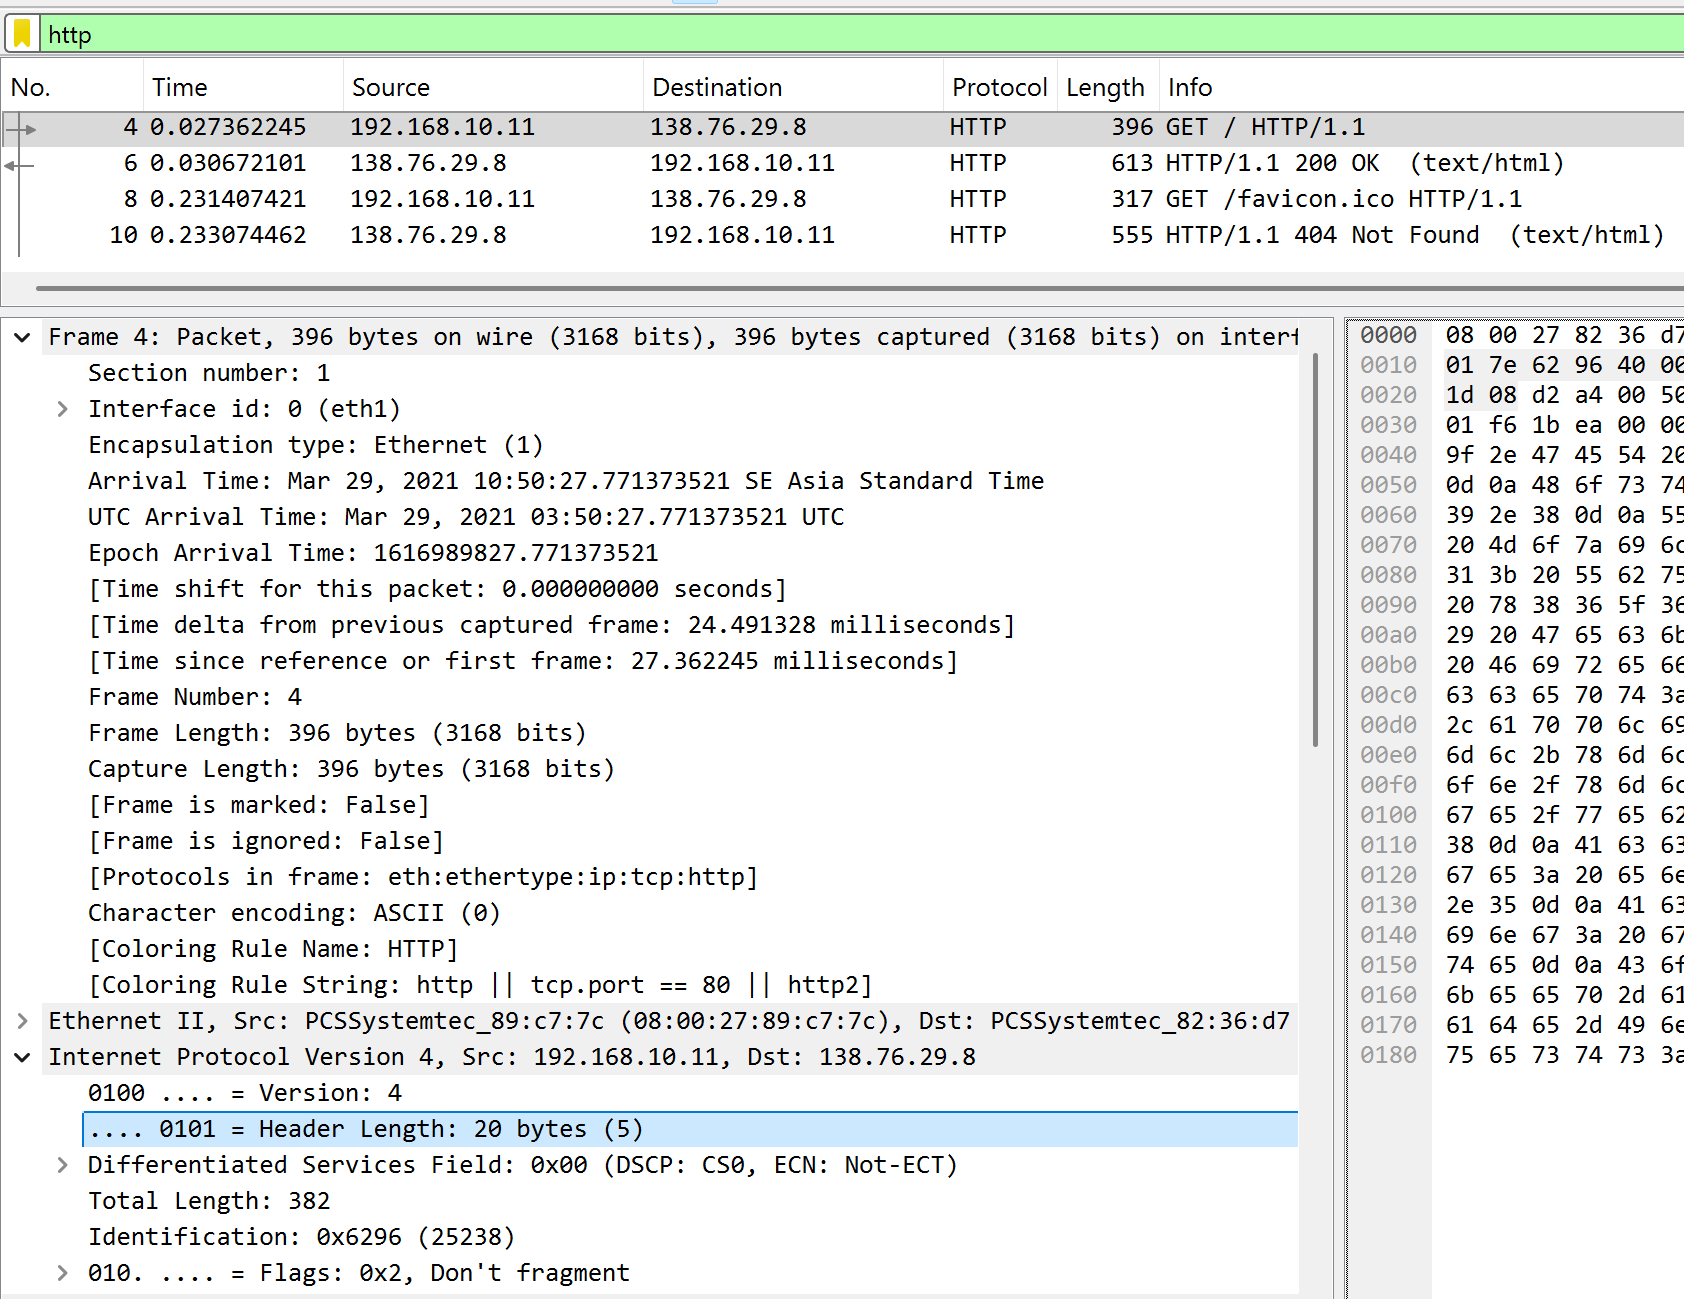
\includegraphics[width=0.58\linewidth]{graphics/fig4_1(2).png}
    \caption{}
\end{figure}

\section{Question 5:}
\textbf{Question:} What are the source and destination IP addresses and TCP source and destination port numbers on the IP datagram carrying this HTTP GET (as recorded in the \textit{nat-outside-wireshark-trace1-1.pcapng} trace file)?

\textbf{Answer:} In packet number 4:
\begin{itemize}[noitemsep]
    \item \textbf{Source IP address:} \texttt{10.0.1.254} (the NAT router's public/WAN IP address)
    \item \textbf{Destination IP address:} \texttt{138.76.29.8}
    \item \textbf{TCP Source port:} \texttt{53924}
    \item \textbf{TCP Destination port:} \texttt{80}
\end{itemize}

\begin{figure}[H]
    \centering
    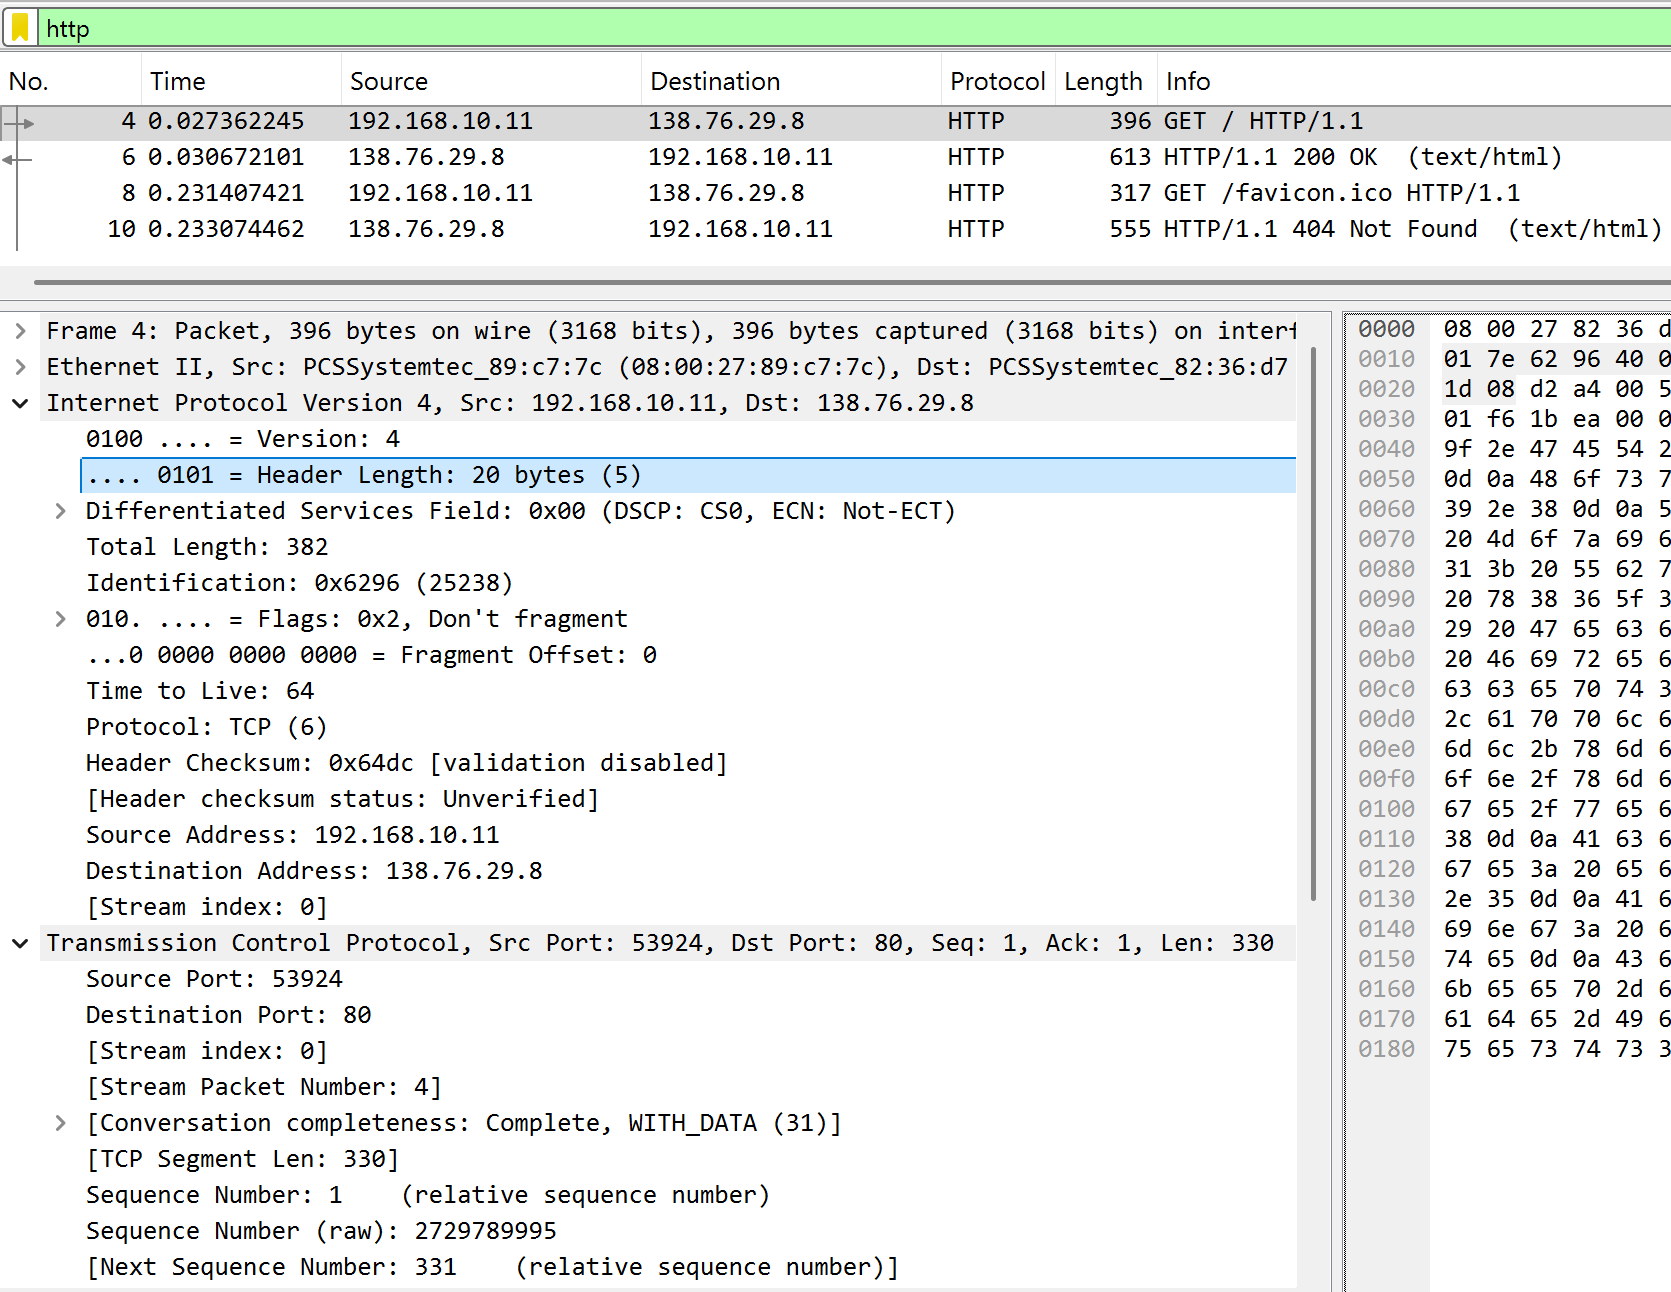
\includegraphics[width=0.58\linewidth]{graphics/fig4_2.png}
    \caption{}
\end{figure}

\section{Question 6:}
\textbf{Question:} Which of these four fields are different than in your answer to question 1 above?

\textbf{Answer:} Comparing the four fields between Question 1 (LAN side) and Question 5 (Internet side):
\begin{itemize}[noitemsep]
    \item \textbf{Source IP address:} \textbf{Different} (\texttt{192.168.10.11} on LAN side vs. \texttt{10.0.1.254} on Internet side). The NAT router translated the private IP address of the internal host into its own WAN IP address.
    \item \textbf{Destination IP address:} \textbf{Same} (\texttt{138.76.29.8} in both traces).
    \item \textbf{TCP Source port:} \textbf{Same} (\texttt{53924} in both traces). Port translation was not necessary because port 53924 was available in the NAT translation table.
    \item \textbf{TCP Destination port:} \textbf{Same} (\texttt{80} in both traces).
\end{itemize}
Therefore, only the \textbf{Source IP address} field is different.


% ==================== PAGE 5: QUESTION 7 & 8 ====================
\section{Question 7:}
\textbf{Question:} Are any fields in the HTTP GET message changed?

\textbf{Answer:} \textbf{No}, none of the fields in the HTTP GET message are changed.
\begin{itemize}[noitemsep]
    \item The TCP payload length is identical in both traces: \textbf{330 bytes}.
    \item The request line (\texttt{GET / HTTP/1.1}) and all headers (\texttt{Host: 138.76.29.8}, \texttt{User-Agent}, \texttt{Accept}, \texttt{Accept-Language}, etc.) are still the same.
\end{itemize}
\textbf{Explanation:} NAT operates at the Network layer (Layer 3) and Transport layer (Layer 4). It modifies IP headers and transport port numbers (along with checksums) without altering the application-layer payload.

\begin{figure}[H]
    \centering
    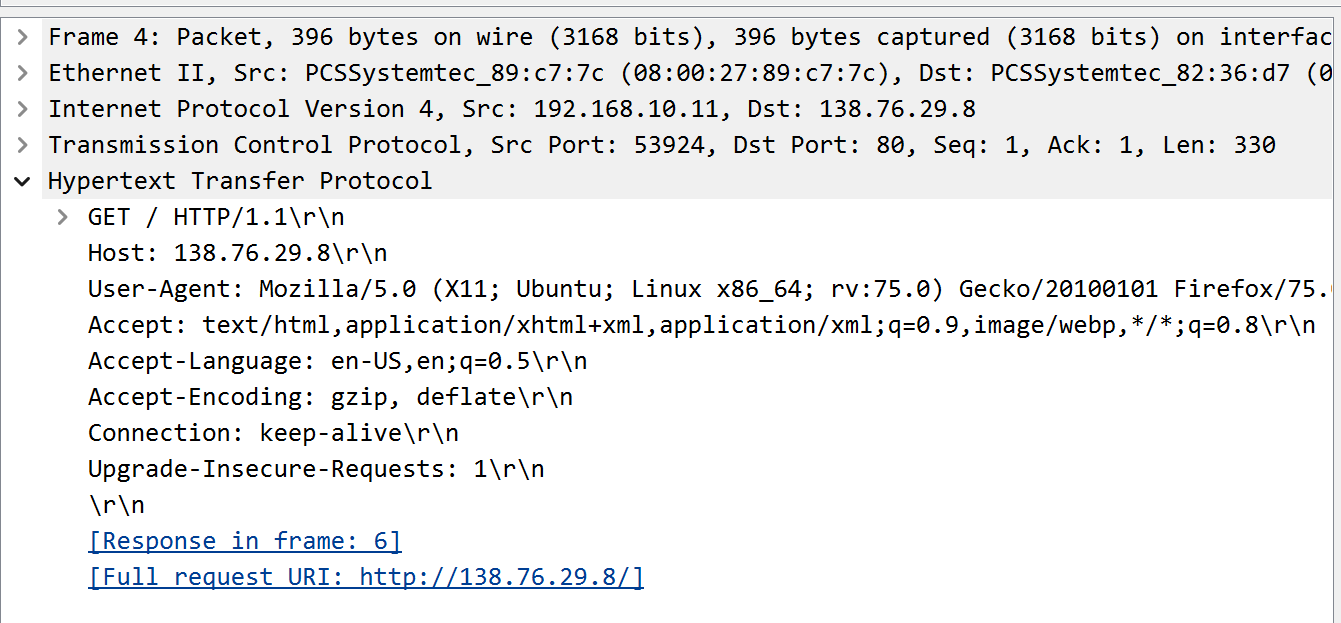
\includegraphics[width=0.49\linewidth]{graphics/fig7_1(1).png}\hfill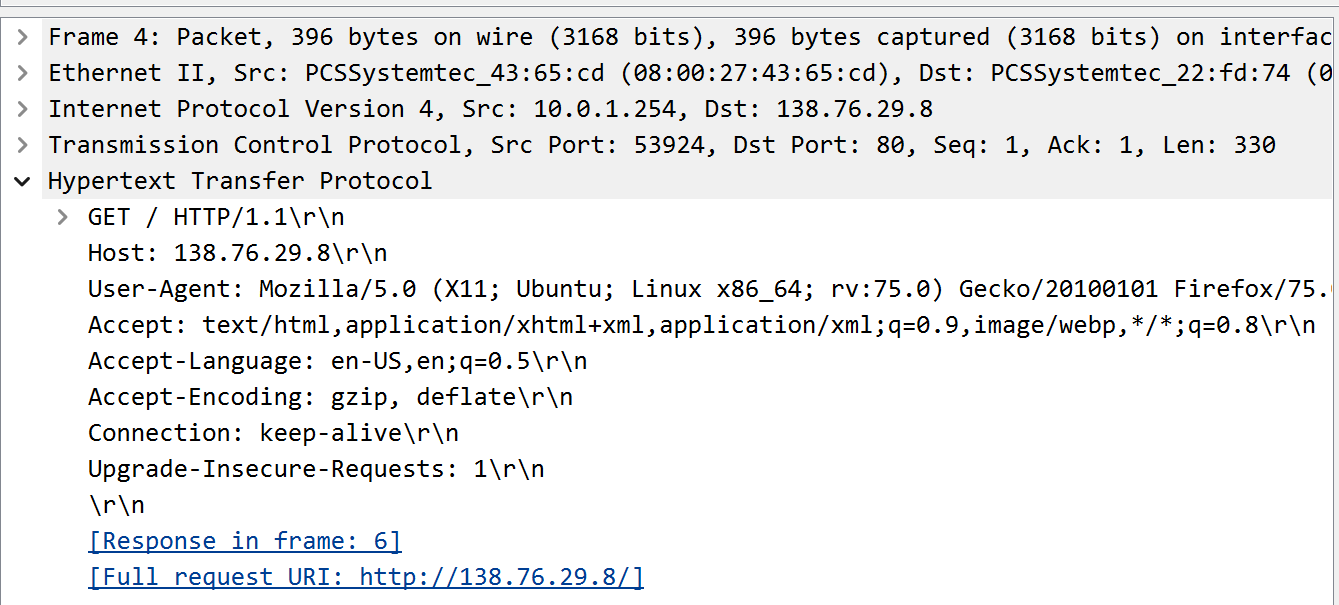
\includegraphics[width=0.49\linewidth]{graphics/fig7_1(2).png}
    \caption{}
\end{figure}

\section{Question 8:}
\textbf{Question:} Which of the following fields in the IP datagram carrying the HTTP GET are changed from the datagram received on the local area network (inside) to the corresponding datagram forwarded on the Internet side (outside) of the NAT router: Version, Header Length, Flags, Checksum?

\textbf{Answer:} Comparing the IP datagram fields of Packet 4 in \textit{nat-inside-wireshark-trace1-1.pcapng} and \textit{nat-outside-wireshark-trace1-1.pcapng}:
\begin{itemize}[noitemsep]
    \item \textbf{Version:} \textbf{Unchanged} (both are IPv4, value \texttt{4}).
    \item \textbf{Header Length:} \textbf{Unchanged} (both are \texttt{20 bytes}, value \texttt{5}).
    \item \textbf{Flags:} \textbf{Unchanged} (both have the Don't Fragment bit set: \texttt{0x2}, Don't fragment).
    \item \textbf{Checksum:} \textbf{Changed} (inside checksum is \texttt{0x64dc}; outside checksum is \texttt{0x2492}).
\end{itemize}
\textbf{Explanation:} The IP header checksum covers the entire IP header. Because the NAT router changes the Source IP address from \texttt{192.168.10.11} to \texttt{10.0.1.254} and decrements the TTL (from 64 to 63), the IP header checksum must be recomputed. Therefore, among the four specified fields, \textbf{only Checksum is changed}.

\begin{figure}[H]
    \centering
    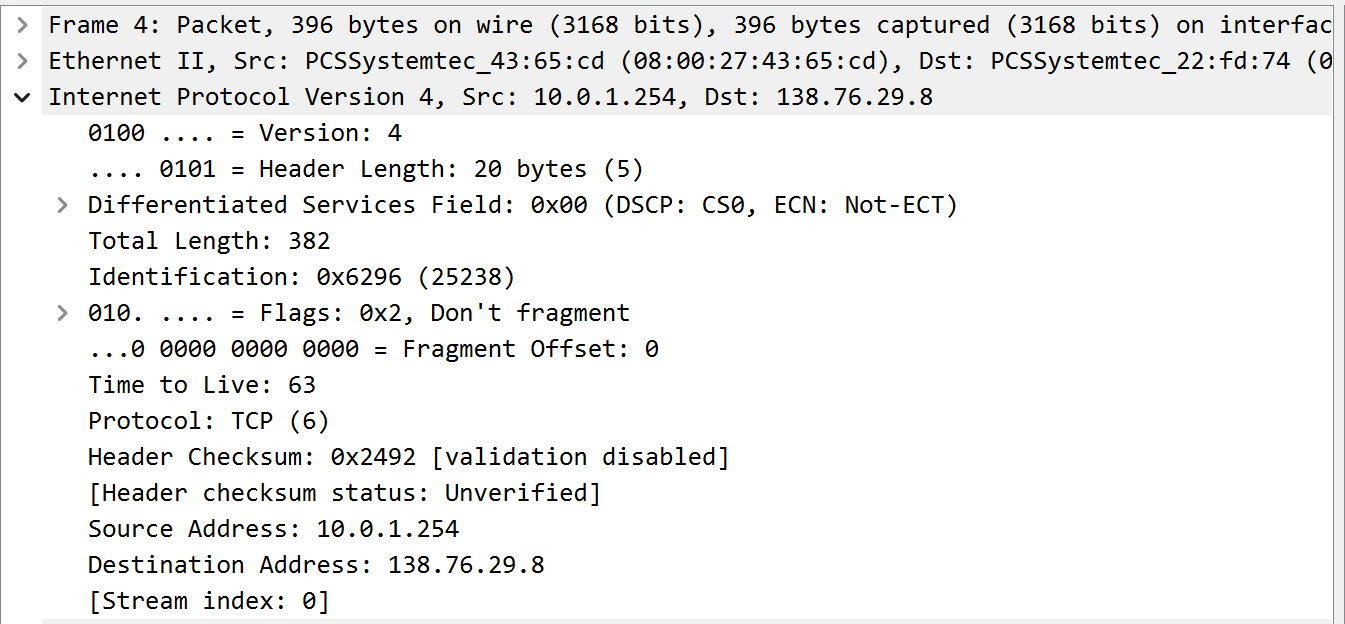
\includegraphics[width=0.70\linewidth]{graphics/fig8_1(1).png}
    \caption{}
\end{figure}


% ==================== PAGE 6: QUESTION 9 & 10 ====================
\section{Question 9:}
\textbf{Question:} At what time does this message appear in the \textit{nat-outside-wireshark-trace1-1.pcapng} trace file?

\textbf{Answer:} In \textit{nat-outside-wireshark-trace1-1.pcapng}, the HTTP 200 OK reply message is packet number 6.
It appears in the trace at time \textbf{0.030626 seconds} (specifically \texttt{0.030625966} seconds relative to the beginning of the trace).

\begin{figure}[H]
    \centering
    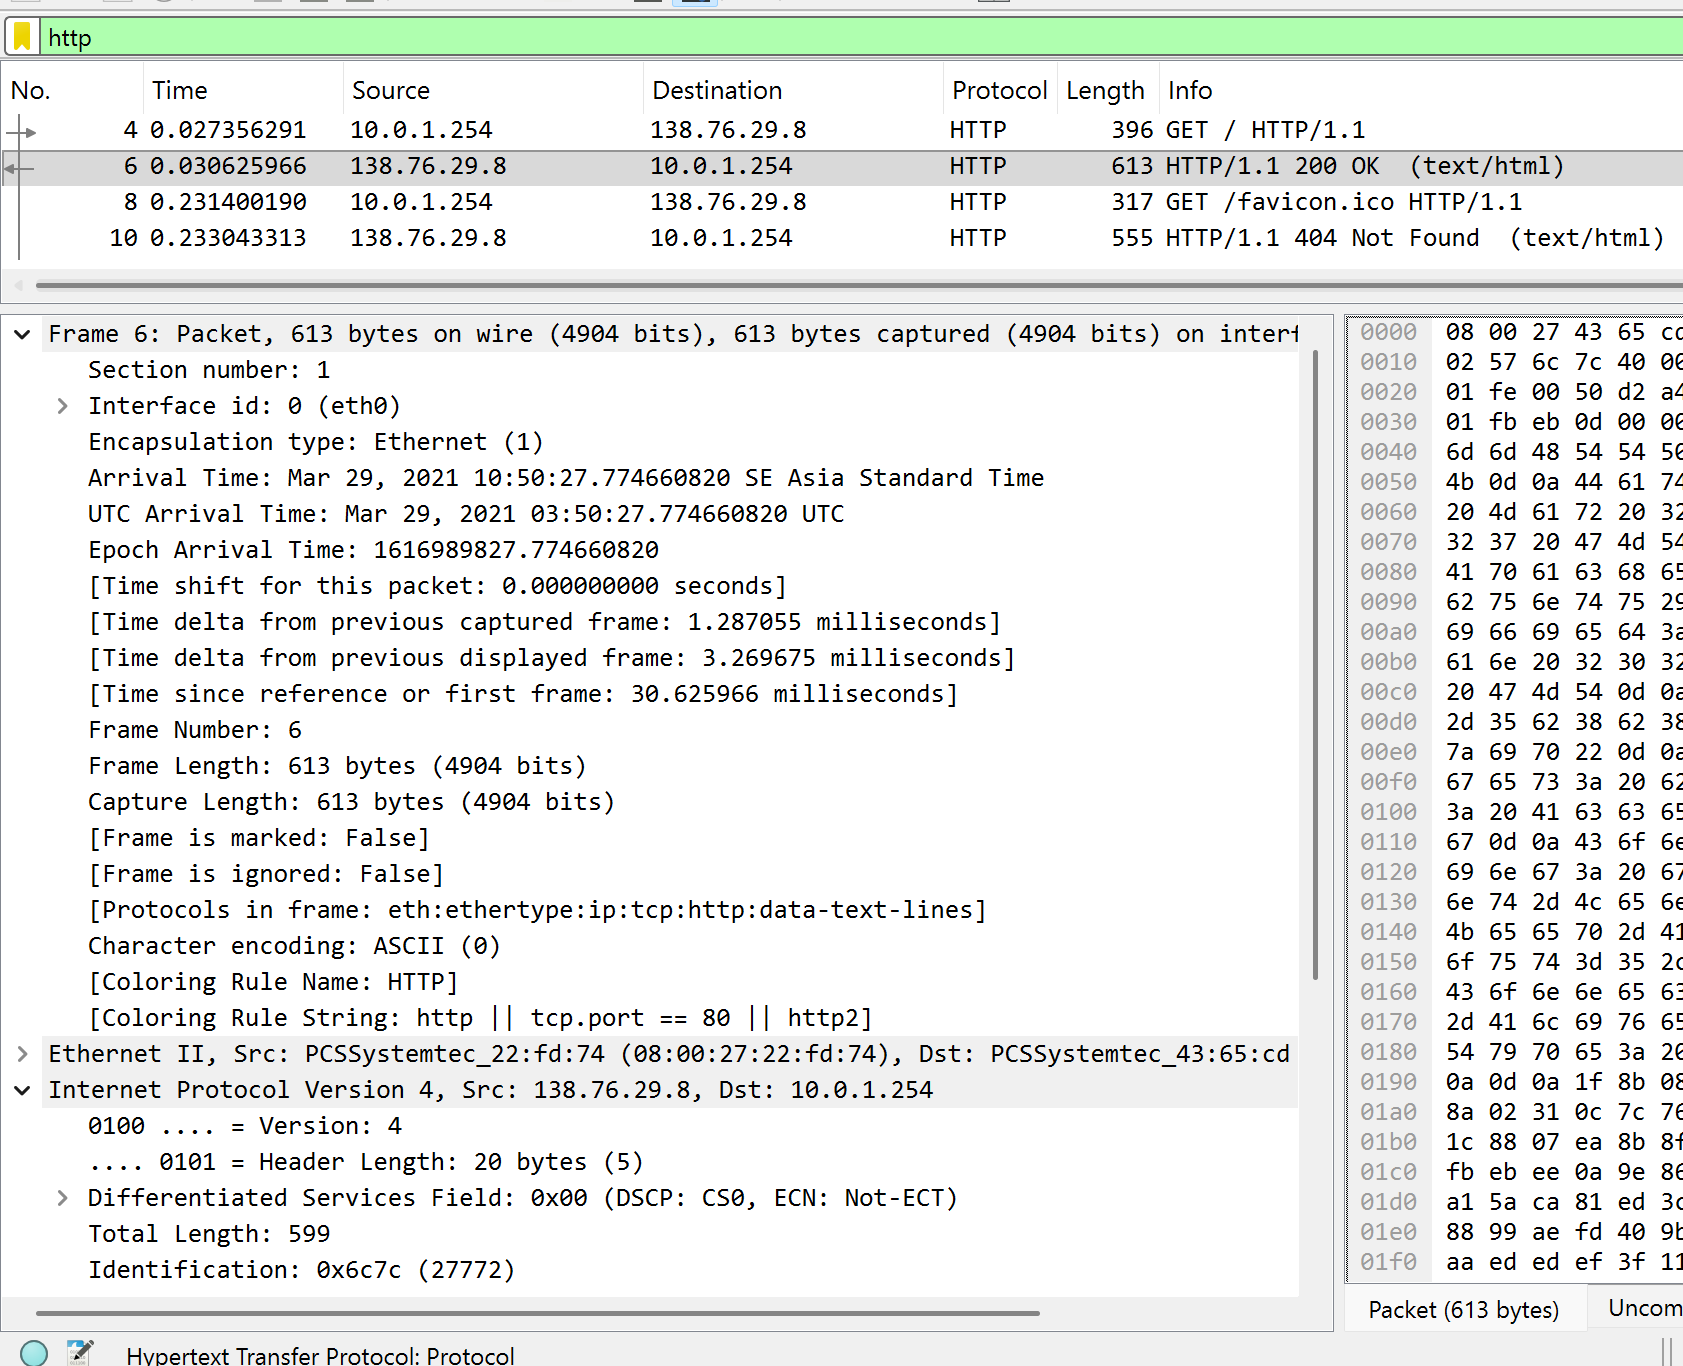
\includegraphics[width=0.58\linewidth]{graphics/fig9_1(1).png}
    \caption{}
\end{figure}

\section{Question 10:}
\textbf{Question:} What are the source and destination IP addresses and TCP source and destination port numbers on the IP datagram carrying this HTTP reply (``200 OK'') message (as recorded in the \textit{nat-outside-wireshark-trace1-1.pcapng} trace file)?

\textbf{Answer:} At packet number 6:
\begin{itemize}[noitemsep]
    \item \textbf{Source IP address:} \texttt{138.76.29.8} (the external web server)
    \item \textbf{Destination IP address:} \texttt{10.0.1.254} (the NAT router's public/WAN IP address)
    \item \textbf{TCP Source port:} \texttt{80}
    \item \textbf{TCP Destination port:} \texttt{53924}
\end{itemize}

\begin{figure}[H]
    \centering
    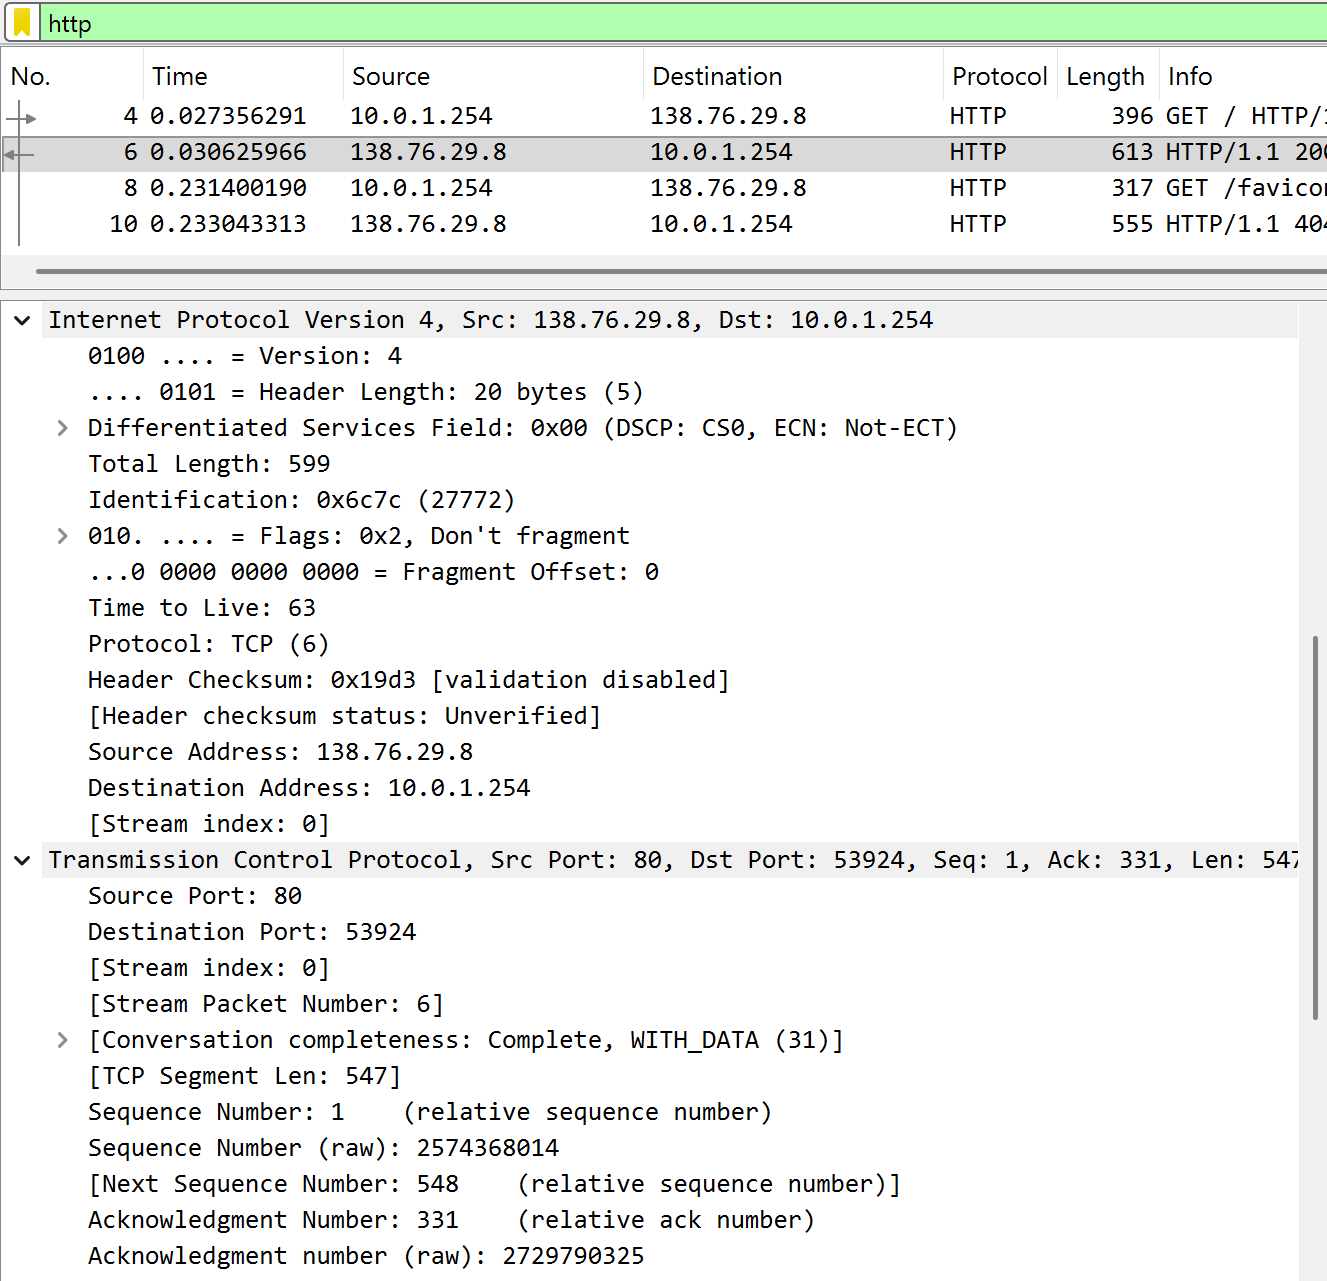
\includegraphics[width=0.58\linewidth]{graphics/fig9_1(2).png}
    \caption{}
\end{figure}


% ==================== PAGE 7: QUESTION 11 ====================
\section{Question 11:}
\textbf{Question:} What are the source and destination IP addresses and TCP source and destination port numbers on the IP datagram carrying the HTTP reply (``200 OK'') that is forwarded from the router to the destination host in the right of Figure 1?

Just to make sure you understand NAT, you should now use Wireshark to peek into the \textit{nat-inside-wireshark-trace1-1.pcapng} trace file at look at the HTTP reply (``200 OK''). Do your answers to question 11 above match what you see in the \textit{nat-inside-wireshark-trace1-1.pcapng} trace file? [Hopefully, your answer is yes :)].

\textbf{Answer:} Based on the operation of NAT, when the inbound reply from the web server arrives at the router:
\begin{itemize}[noitemsep]
    \item The router searches its NAT translation table for an active entry matching destination port \texttt{53924}.
    \item It translates the Destination IP address from its WAN interface (\texttt{10.0.1.254}) back to the private LAN IP address of the client (\texttt{192.168.10.11}).
    \item The Source IP address (\texttt{138.76.29.8}), Source port (\texttt{80}), and Destination port (\texttt{53924}) are left unchanged.
\end{itemize}
Thus, on the IP datagram forwarded to the client host inside the LAN:
\begin{itemize}[noitemsep]
    \item \textbf{Source IP address:} \texttt{138.76.29.8}
    \item \textbf{Destination IP address:} \texttt{192.168.10.11}
    \item \textbf{TCP Source port:} \texttt{80}
    \item \textbf{TCP Destination port:} \texttt{53924}
\end{itemize}

\textbf{Verification:}
Yes! Inspecting packet number 6 in \textit{nat-inside-wireshark-trace1-1.pcapng} (Figure 11.1) confirms that the captured fields (Source IP: \texttt{138.76.29.8}, Destination IP: \texttt{192.168.10.11}, Source Port: \texttt{80}, Destination Port: \texttt{53924}) match our theoretical prediction completely.

\begin{figure}[H]
    \centering
    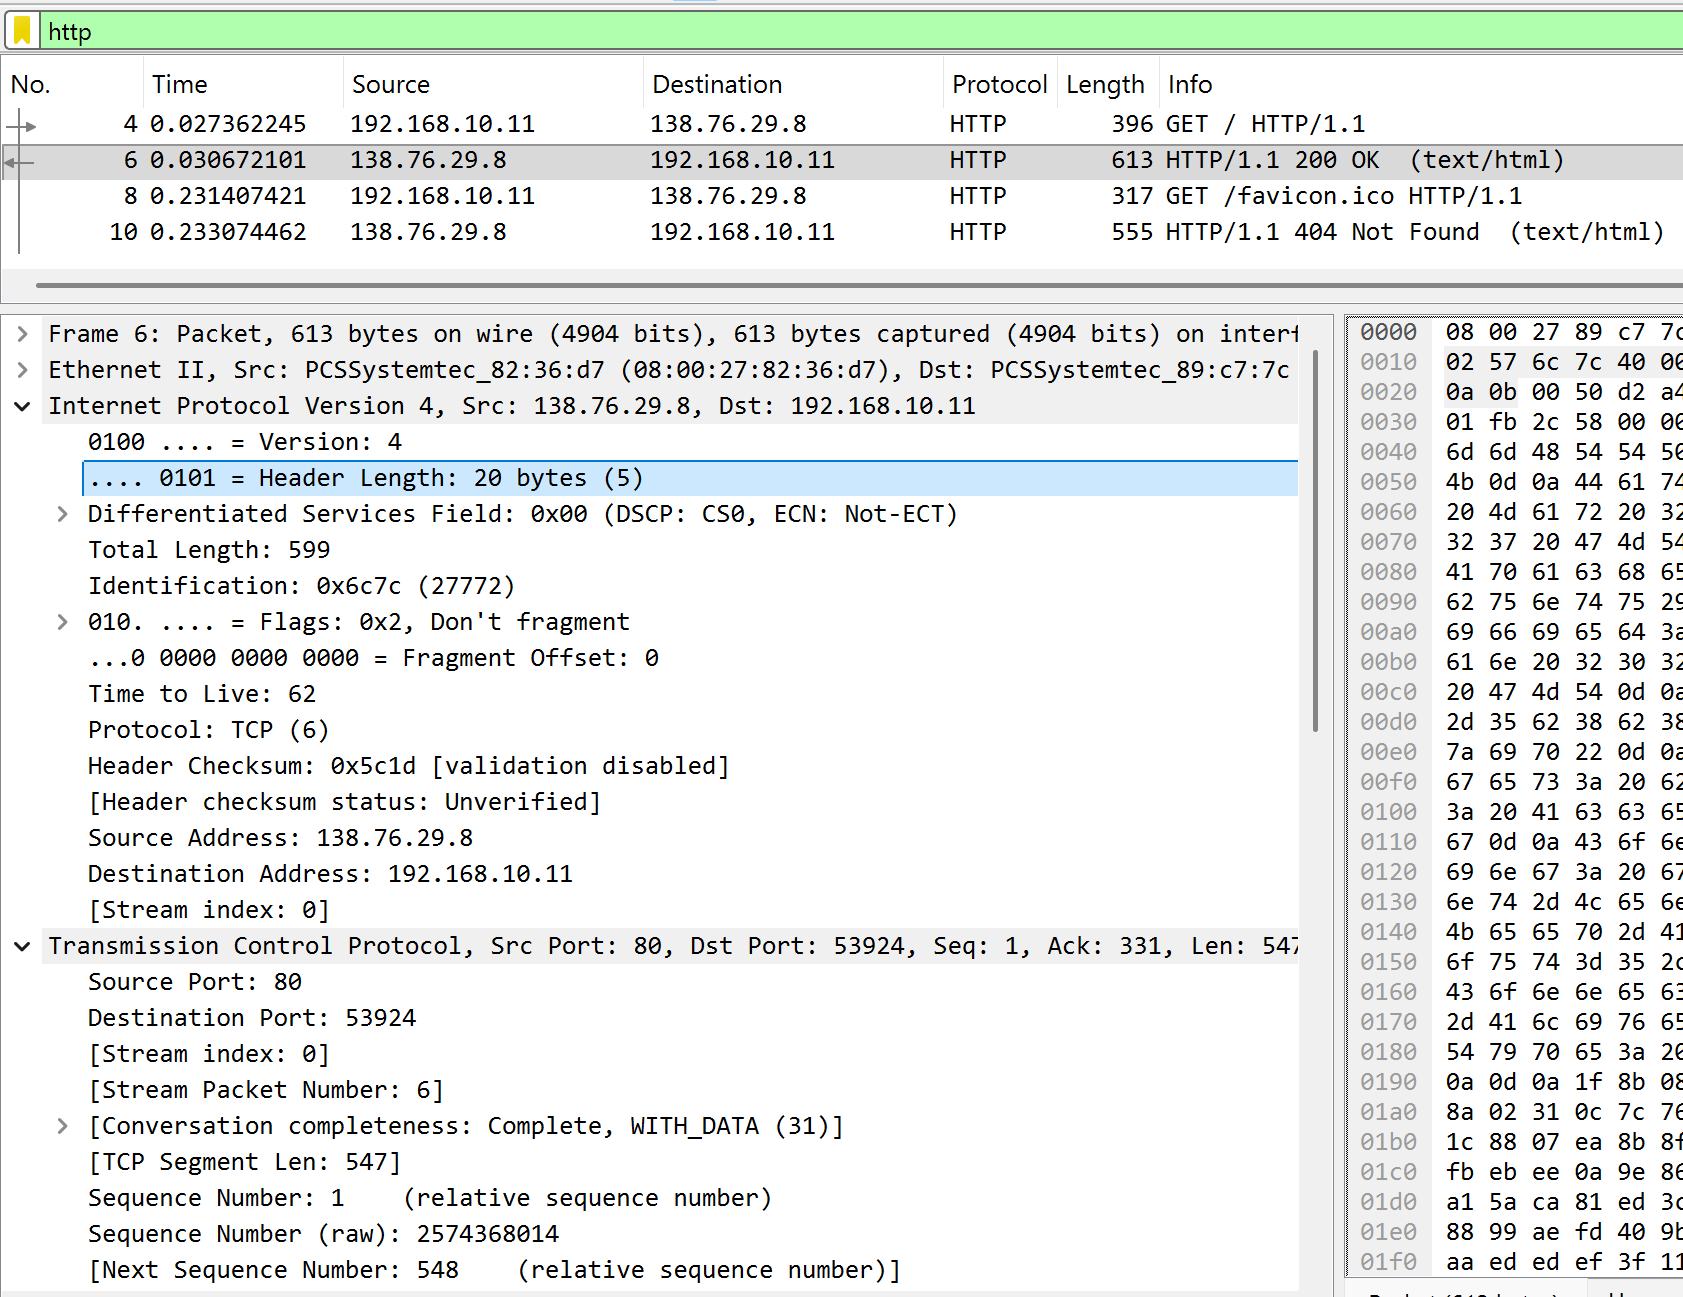
\includegraphics[width=0.58\linewidth]{graphics/fig11_1(1).png}
    \caption{}
\end{figure}

\end{document}
